
\section{Appendix for use in STA 610 (Thesis
II)}\label{appendix-for-use-in-sta-610-thesis-ii}

Data was queried using USGS Earthquake Catalog:
\url{https://earthquake.usgs.gov/earthquakes/search/} to select all
recorded earthquakes of magnitude 4.5 and above with the following query
parameters:

\begin{itemize}
\tightlist
\item
  latitude 35.4 - 41.2
\item
  longitude 137.5 - 145.2
\item
  Timeframe(UTC): 2011-03-11 00:00:00 - 1965-01-01 00:00:00
\end{itemize}

The data was stored locally in a .csv file named \texttt{earthquakes}.

The organization also has an package called \texttt{rcomcat} to query
data directly into \texttt{R}, but its version was not compatible at the
time of this thesis.

\hypertarget{data-preprocessing}{%
\subsection{Data Preprocessing}\label{data-preprocessing}}

\begin{Shaded}
\begin{Highlighting}[]
\CommentTok{\# load the data }
\NormalTok{earthquakes\_full }\OtherTok{\textless{}{-}} \FunctionTok{read.csv}\NormalTok{(}\StringTok{"data/earthquakes.csv"}\NormalTok{)}

\CommentTok{\# subset data to include observations from January 1, 1965 to}
\CommentTok{\#  just before the Greak Quake of March 11, 2011}
\NormalTok{earthquakes\_subset }\OtherTok{\textless{}{-}}\NormalTok{ earthquakes\_full[}\FunctionTok{which}\NormalTok{(earthquakes\_full}\SpecialCharTok{$}\NormalTok{time }\SpecialCharTok{\textgreater{}=} \StringTok{"1965{-}01{-}26T23:47:37.120Z"} \SpecialCharTok{\&}\NormalTok{                                                                      earthquakes\_full}\SpecialCharTok{$}\NormalTok{time }\SpecialCharTok{\textless{}=} \StringTok{"2011{-}03{-}11T05:44:24.120Z"}\NormalTok{),]}
  
\CommentTok{\# fine{-}tune the geographic area of the model}
\NormalTok{earthquakes\_subset }\OtherTok{\textless{}{-}}\NormalTok{ earthquakes\_subset[}\FunctionTok{which}\NormalTok{(earthquakes\_subset}\SpecialCharTok{$}\NormalTok{latitude }\SpecialCharTok{\textgreater{}} \FloatTok{35.72} \SpecialCharTok{\&}
\NormalTok{                                               earthquakes\_subset}\SpecialCharTok{$}\NormalTok{latitude }\SpecialCharTok{\textless{}} \FloatTok{40.82} \SpecialCharTok{\&}
\NormalTok{                                               earthquakes\_subset}\SpecialCharTok{$}\NormalTok{longitude }\SpecialCharTok{\textgreater{}} \FloatTok{139.37} \SpecialCharTok{\&}
\NormalTok{                                               earthquakes\_subset}\SpecialCharTok{$}\NormalTok{longitude }\SpecialCharTok{\textless{}} \FloatTok{143.37}\NormalTok{),]}

\CommentTok{\# data frame of magnitudes (rounded to .1) and relative frequencies}
\NormalTok{eq }\OtherTok{\textless{}{-}} \FunctionTok{data.frame}\NormalTok{(}\FunctionTok{table}\NormalTok{(}\FunctionTok{round}\NormalTok{(earthquakes\_subset}\SpecialCharTok{$}\NormalTok{mag, }\DecValTok{1}\NormalTok{)) ) }\SpecialCharTok{\%\textgreater{}\%} 
                 \FunctionTok{rename}\NormalTok{(}\AttributeTok{mag =}\NormalTok{ Var1,}
                       \AttributeTok{freq =}\NormalTok{ Freq) }\SpecialCharTok{\%\textgreater{}\%} 
                 \FunctionTok{mutate}\NormalTok{(}\AttributeTok{mag =} \FunctionTok{as.numeric}\NormalTok{(}\FunctionTok{as.character}\NormalTok{(mag))) }\SpecialCharTok{\%\textgreater{}\%} \CommentTok{\#change to numeric rather than factors}
                 \FunctionTok{mutate}\NormalTok{(}\AttributeTok{freq =}\NormalTok{ freq}\SpecialCharTok{/}\NormalTok{(}\DecValTok{2011{-}1965}\NormalTok{))      }\CommentTok{\#AVERAGE annual frequencies over the 46{-}year span}

\CommentTok{\# create a new variable representing the frequency of earthquakes of AT LEAST that magnitude}
\ControlFlowTok{for}\NormalTok{(i }\ControlFlowTok{in} \DecValTok{1}\SpecialCharTok{:}\FunctionTok{as.numeric}\NormalTok{(}\FunctionTok{count}\NormalTok{(eq)))\{}
\NormalTok{  eq}\SpecialCharTok{$}\NormalTok{freqc[i] }\OtherTok{\textless{}{-}} \FunctionTok{sum}\NormalTok{( eq}\SpecialCharTok{$}\NormalTok{freq[}\FunctionTok{c}\NormalTok{(i}\SpecialCharTok{:}\FunctionTok{as.numeric}\NormalTok{(}\FunctionTok{count}\NormalTok{(eq)))] )}
\NormalTok{\}}
\end{Highlighting}
\end{Shaded}

\hypertarget{traintest-split}{%
\subsection{Train/Test Split}\label{traintest-split}}

\begin{Shaded}
\begin{Highlighting}[]
\CommentTok{\# shuffle the data}
\NormalTok{df }\OtherTok{\textless{}{-}}\NormalTok{ eq[}\FunctionTok{sample}\NormalTok{(}\FunctionTok{nrow}\NormalTok{(eq)), ]}

\CommentTok{\# Extract 80\% of data into train set and the remaining 30\% in test set}
\NormalTok{train\_test\_split }\OtherTok{\textless{}{-}} \FloatTok{0.8} \SpecialCharTok{*} \FunctionTok{nrow}\NormalTok{(df)}
\NormalTok{train }\OtherTok{\textless{}{-}}\NormalTok{ df[}\DecValTok{1}\SpecialCharTok{:}\NormalTok{train\_test\_split,]}
\NormalTok{test }\OtherTok{\textless{}{-}}\NormalTok{ df[(train\_test\_split}\SpecialCharTok{+}\DecValTok{1}\NormalTok{)}\SpecialCharTok{:} \FunctionTok{nrow}\NormalTok{(df),]}

\NormalTok{test}\SpecialCharTok{$}\NormalTok{set }\OtherTok{\textless{}{-}} \StringTok{"test"}
\NormalTok{train}\SpecialCharTok{$}\NormalTok{set }\OtherTok{\textless{}{-}} \StringTok{"train"}
\end{Highlighting}
\end{Shaded}

\hypertarget{traditional-poisson-regression-model}{%
\subsection{Traditional Poisson Regression
Model}\label{traditional-poisson-regression-model}}

\begin{Shaded}
\begin{Highlighting}[]
\NormalTok{pois }\OtherTok{\textless{}{-}} \FunctionTok{glm}\NormalTok{(freqc }\SpecialCharTok{\textasciitilde{}}\NormalTok{ mag, }\AttributeTok{data =}\NormalTok{ train, }\AttributeTok{family =} \StringTok{"poisson"}\NormalTok{)}
\FunctionTok{summary}\NormalTok{(pois)}
\end{Highlighting}
\end{Shaded}

\begin{verbatim}
## 
## Call:
## glm(formula = freqc ~ mag, family = "poisson", data = train)
## 
## Deviance Residuals: 
##      Min        1Q    Median        3Q       Max  
## -0.39403  -0.20754  -0.02925   0.08617   0.22166  
## 
## Coefficients:
##             Estimate Std. Error z value Pr(>|z|)    
## (Intercept)  13.0940     0.7242   18.08   <2e-16 ***
## mag          -2.0467     0.1474  -13.88   <2e-16 ***
## ---
## Signif. codes:  0 '***' 0.001 '**' 0.01 '*' 0.05 '.' 0.1 ' ' 1
## 
## (Dispersion parameter for poisson family taken to be 1)
## 
##     Null deviance: 373.0667  on 23  degrees of freedom
## Residual deviance:   0.7758  on 22  degrees of freedom
## AIC: Inf
## 
## Number of Fisher Scoring iterations: 3
\end{verbatim}

\begin{Shaded}
\begin{Highlighting}[]
\CommentTok{\#{-}{-}{-}append relevant predictions to the training and test datasets}
\NormalTok{train}\SpecialCharTok{$}\NormalTok{fitted }\OtherTok{\textless{}{-}} \FunctionTok{predict}\NormalTok{(pois, }\AttributeTok{type =} \StringTok{"response"}\NormalTok{)}
\NormalTok{test}\SpecialCharTok{$}\NormalTok{fitted }\OtherTok{\textless{}{-}} \FunctionTok{predict}\NormalTok{(pois, }\AttributeTok{type =} \StringTok{"response"}\NormalTok{, }\AttributeTok{newdata =} \FunctionTok{data.frame}\NormalTok{(}\AttributeTok{mag =}\NormalTok{ test}\SpecialCharTok{$}\NormalTok{mag))}

\CommentTok{\#{-}{-}combine data sets for plot}
\NormalTok{plot }\OtherTok{\textless{}{-}}\NormalTok{ train[,}\FunctionTok{c}\NormalTok{(}\StringTok{"mag"}\NormalTok{,}\StringTok{"freqc"}\NormalTok{,}\StringTok{"set"}\NormalTok{,}\StringTok{"fitted"}\NormalTok{)] }\SpecialCharTok{\%\textgreater{}\%}
            \FunctionTok{rbind}\NormalTok{(test[,}\FunctionTok{c}\NormalTok{(}\StringTok{"mag"}\NormalTok{,}\StringTok{"freqc"}\NormalTok{,}\StringTok{"set"}\NormalTok{,}\StringTok{"fitted"}\NormalTok{)])}

\CommentTok{\#{-}{-}{-}plot the data}
\FunctionTok{ggplot}\NormalTok{(plot, }\FunctionTok{aes}\NormalTok{(}\AttributeTok{x =}\NormalTok{ mag)) }\SpecialCharTok{+}
  \FunctionTok{geom\_point}\NormalTok{(}\AttributeTok{size =} \DecValTok{4}\NormalTok{, }\AttributeTok{shape =} \DecValTok{17}\NormalTok{, }\FunctionTok{aes}\NormalTok{(}\AttributeTok{y =}\NormalTok{ freqc, }\AttributeTok{color =}\NormalTok{ set)) }\SpecialCharTok{+}
  \FunctionTok{geom\_smooth}\NormalTok{(}\FunctionTok{aes}\NormalTok{(}\AttributeTok{y =}\NormalTok{ fitted), }\AttributeTok{size =}\NormalTok{ .}\DecValTok{2}\NormalTok{, }\AttributeTok{alpha =}\NormalTok{ .}\DecValTok{2}\NormalTok{) }\SpecialCharTok{+}
  \FunctionTok{theme\_minimal}\NormalTok{() }\SpecialCharTok{+}
  \FunctionTok{labs}\NormalTok{(}\AttributeTok{x =} \StringTok{"Magnitude"}\NormalTok{,}
       \AttributeTok{y =} \StringTok{"Annual Frequency of At Least this Magnitude"}\NormalTok{,}
       \AttributeTok{title =} \StringTok{"Annual Earthquake Frequency near Tohoku, Japan"}\NormalTok{,}
       \AttributeTok{subtitle =} \StringTok{"Poisson Regression Model"}\NormalTok{)}
\end{Highlighting}
\end{Shaded}

\begin{verbatim}
## `geom_smooth()` using method = 'loess' and formula = 'y ~ x'
\end{verbatim}

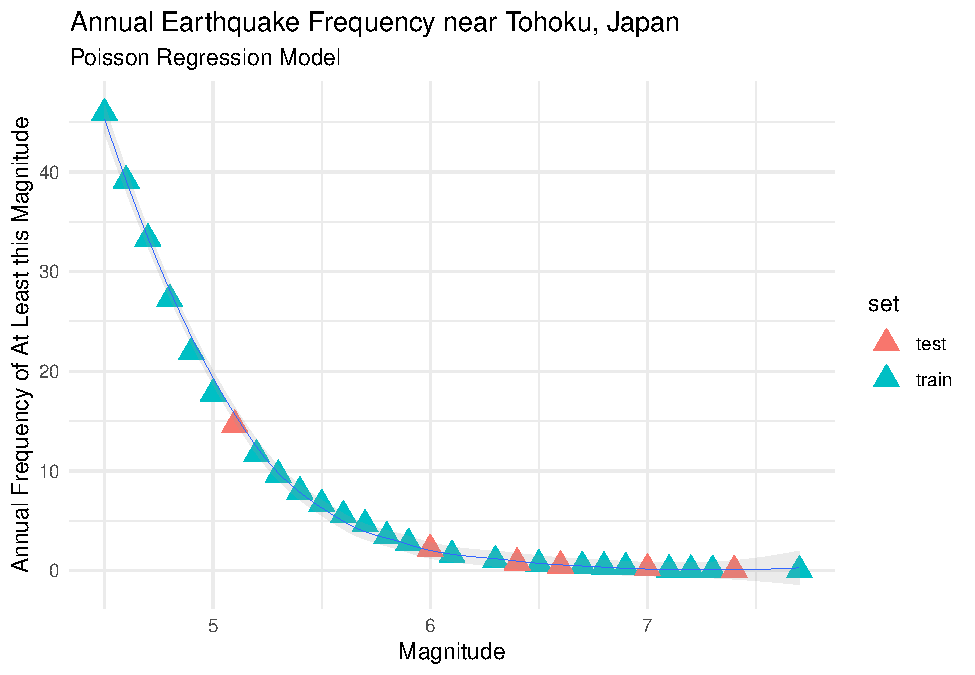
\includegraphics{Appendix_eq_files/figure-latex/unnamed-chunk-3-1.pdf}

\begin{Shaded}
\begin{Highlighting}[]
\CommentTok{\# }\AlertTok{TEST}\CommentTok{ ERROR {-} MSE}
\NormalTok{poissontable }\OtherTok{\textless{}{-}} \FunctionTok{data.frame}\NormalTok{(}\AttributeTok{Model =} \StringTok{"Poisson Regression"}\NormalTok{,}
                          \CommentTok{\# Hidden = NA,}
                           \AttributeTok{TestErr =} \FunctionTok{mean}\NormalTok{((test}\SpecialCharTok{$}\NormalTok{freqc }\SpecialCharTok{{-}}\NormalTok{ test}\SpecialCharTok{$}\NormalTok{fitted)}\SpecialCharTok{\^{}}\DecValTok{2}\NormalTok{))}
                           \CommentTok{\#TrainErr =  sum((pois[["residuals"]])\^{}2))}
\NormalTok{poissontable}
\end{Highlighting}
\end{Shaded}

\begin{verbatim}
##                Model    TestErr
## 1 Poisson Regression 0.03940496
\end{verbatim}

\hypertarget{multi-layer-perceptron}{%
\subsection{\#\# Multi-Layer Perceptron}\label{multi-layer-perceptron}}

Cross validation scheme to measure MLP hidden layer size. Due to the
size of the data, distributions of TestError were skewed. So, median was
taken to measure the final CV score for the network.

It is found that the network converges faster on the log scale, so the
data is transformed first.

\begin{Shaded}
\begin{Highlighting}[]
\NormalTok{k }\OtherTok{\textless{}{-}} \DecValTok{20}
\NormalTok{TestErr }\OtherTok{\textless{}{-}} \ConstantTok{NULL}
\NormalTok{H }\OtherTok{\textless{}{-}} \ConstantTok{NULL}
\NormalTok{H\_med }\OtherTok{\textless{}{-}} \ConstantTok{NULL}

\ControlFlowTok{for}\NormalTok{(j }\ControlFlowTok{in} \FunctionTok{c}\NormalTok{(}\DecValTok{3}\NormalTok{,}\DecValTok{6}\NormalTok{,}\DecValTok{9}\NormalTok{,}\DecValTok{10}\NormalTok{,}\DecValTok{20}\NormalTok{))\{}

  \ControlFlowTok{for}\NormalTok{(i }\ControlFlowTok{in} \DecValTok{1}\SpecialCharTok{:}\NormalTok{k)\{}
\NormalTok{    df }\OtherTok{\textless{}{-}}\NormalTok{ eq[}\FunctionTok{sample}\NormalTok{(}\FunctionTok{nrow}\NormalTok{(eq)), ]}

    \CommentTok{\# Extract 70\% of data into train set and the remaining 30\% in test set}
\NormalTok{    train\_test\_split }\OtherTok{\textless{}{-}} \FloatTok{0.7} \SpecialCharTok{*} \FunctionTok{nrow}\NormalTok{(df)}
\NormalTok{    train }\OtherTok{\textless{}{-}}\NormalTok{ df[}\DecValTok{1}\SpecialCharTok{:}\NormalTok{train\_test\_split,]}
\NormalTok{    test }\OtherTok{\textless{}{-}}\NormalTok{ df[(train\_test\_split}\SpecialCharTok{+}\DecValTok{1}\NormalTok{)}\SpecialCharTok{:} \FunctionTok{nrow}\NormalTok{(df),]}

\NormalTok{    train}\SpecialCharTok{$}\NormalTok{freqc\_log }\OtherTok{\textless{}{-}} \FunctionTok{log10}\NormalTok{(train}\SpecialCharTok{$}\NormalTok{freqc) }\CommentTok{\#log transform for faster convergence}
    \CommentTok{\# test$set \textless{}{-} "test"}
    \CommentTok{\# train$set \textless{}{-} "train"}

\NormalTok{    mlp }\OtherTok{\textless{}{-}} \FunctionTok{neuralnet}\NormalTok{(freqc\_log }\SpecialCharTok{\textasciitilde{}}\NormalTok{ mag,}
                     \AttributeTok{stepmax =} \FloatTok{1e+06}\NormalTok{,}
                     \AttributeTok{data =}\NormalTok{ train,}
                     \AttributeTok{hidden =} \FunctionTok{c}\NormalTok{(j))}

    \CommentTok{\#{-}{-}{-}exponentiate predictions to coerce back to standard scale}
\NormalTok{    testpreds }\OtherTok{\textless{}{-}} \DecValTok{10}\SpecialCharTok{\^{}}\FunctionTok{predict}\NormalTok{(mlp,}\AttributeTok{newdata =} \FunctionTok{data.frame}\NormalTok{(}\AttributeTok{mag =}\NormalTok{ test}\SpecialCharTok{$}\NormalTok{mag))}

    \CommentTok{\#{-}{-}{-}Mean difference between prediction and actual values for test set}
\NormalTok{    TestErr[i] }\OtherTok{\textless{}{-}} \FunctionTok{mean}\NormalTok{((test}\SpecialCharTok{$}\NormalTok{freqc }\SpecialCharTok{{-}}\NormalTok{ testpreds)}\SpecialCharTok{\^{}}\DecValTok{2}\NormalTok{) }
\NormalTok{  \}}

\NormalTok{H\_med[j] }\OtherTok{\textless{}{-}} \FunctionTok{median}\NormalTok{(TestErr)}

\NormalTok{\}}


\NormalTok{mlptable\_cv }\OtherTok{\textless{}{-}} \FunctionTok{na.omit}\NormalTok{(}\FunctionTok{data.frame}\NormalTok{(}\AttributeTok{Model =} \StringTok{"MLP"}\NormalTok{, }\AttributeTok{TestErr =}\NormalTok{ H\_med))}
\NormalTok{mlptable\_cv}
\end{Highlighting}
\end{Shaded}

\begin{verbatim}
##    Model   TestErr
## 3    MLP 0.1859479
## 6    MLP 0.2940994
## 9    MLP 0.5004098
## 10   MLP 0.3152632
## 20   MLP 0.8421863
\end{verbatim}

\hypertarget{note-on-mlp-for-count-data}{%
\subsubsection{Note on MLP for count
data}\label{note-on-mlp-for-count-data}}

It is worth noting here that a comparable MLP model to Poisson
regression may be more appropriate for the task at hand. Particularly,
the networks used in \cite{fallah2009nonlinear} to compare the
performance of a neural network Poisson regression model with its
traditional counterpart among various data sets were attempted for this
example. According to the paper, a two-layer neural network is used that
uses hyperbolic tangent in the hidden layer and the exponential function
in the output. To accommodate count data, the loss function based on
negative log likelihood criterion for Poisson regression is: \[
E_D = - \sum_{i=1}^N \left[ -\hat{y_i} + y_i log(\hat{y_i}) \right]
\]

And so the code for the \texttt{neuralnets} package would look as
follows:

\begin{Shaded}
\begin{Highlighting}[]
\NormalTok{mlp }\OtherTok{\textless{}{-}} \FunctionTok{neuralnet}\NormalTok{(freqc }\SpecialCharTok{\textasciitilde{}}\NormalTok{ mag,}
                 \AttributeTok{stepmax =} \FloatTok{1e+06}\NormalTok{,}
                 \AttributeTok{data =}\NormalTok{ train,}
                 \AttributeTok{hidden =} \FunctionTok{c}\NormalTok{(}\DecValTok{5}\NormalTok{),}
                 \AttributeTok{act.fct =} \StringTok{"tanh"}\NormalTok{,}
                 \AttributeTok{err.fct =} \ControlFlowTok{function}\NormalTok{(x, y) \{ }\SpecialCharTok{{-}}\NormalTok{(}\SpecialCharTok{{-}}\NormalTok{x}\SpecialCharTok{+}\NormalTok{y}\SpecialCharTok{*}\FunctionTok{log}\NormalTok{(x))\})}

\NormalTok{predictions }\OtherTok{\textless{}{-}} \FunctionTok{predict}\NormalTok{(mlp, }\AttributeTok{newdata =} \FunctionTok{data.frame}\NormalTok{(}\AttributeTok{mag =}\NormalTok{ test}\SpecialCharTok{$}\NormalTok{mag)) }\SpecialCharTok{\%\textgreater{}\%} \FunctionTok{exp}\NormalTok{()}
\end{Highlighting}
\end{Shaded}

\hypertarget{bayesian-reguarized-neural-network}{%
\subsection{Bayesian Reguarized Neural
Network}\label{bayesian-reguarized-neural-network}}

Using the \texttt{brnn} package \cite{brnn} to create a two-layer neural
network with 6 hidden neurons. Network uses Bayesian regularization to
set parameters \(\alpha\) and \(\beta\).

\begin{Shaded}
\begin{Highlighting}[]
\NormalTok{x }\OtherTok{\textless{}{-}}\NormalTok{ train}\SpecialCharTok{$}\NormalTok{mag}
\NormalTok{y }\OtherTok{\textless{}{-}}\NormalTok{ train}\SpecialCharTok{$}\NormalTok{freqc}
\NormalTok{TestErr }\OtherTok{\textless{}{-}} \ConstantTok{NULL}
\NormalTok{TrainErr }\OtherTok{\textless{}{-}} \ConstantTok{NULL}
\NormalTok{Hidden }\OtherTok{\textless{}{-}} \ConstantTok{NULL}

\ControlFlowTok{for}\NormalTok{(i }\ControlFlowTok{in} \FunctionTok{c}\NormalTok{(}\DecValTok{3}\NormalTok{,}\DecValTok{6}\NormalTok{,}\DecValTok{9}\NormalTok{,}\DecValTok{10}\NormalTok{,}\DecValTok{20}\NormalTok{))\{}

\CommentTok{\#{-}{-}{-}build the model with hidden layer size i}
\NormalTok{brnn }\OtherTok{\textless{}{-}} \FunctionTok{brnn}\NormalTok{(y}\SpecialCharTok{\textasciitilde{}}\NormalTok{x,}\AttributeTok{neurons=}\NormalTok{i)}

\CommentTok{\#{-}{-}{-}exponentiate predictions to coerce back to standard scale}
\NormalTok{testpreds }\OtherTok{\textless{}{-}} \FunctionTok{predict}\NormalTok{(brnn, }\AttributeTok{newdata =} \FunctionTok{data.frame}\NormalTok{(}\AttributeTok{x =}\NormalTok{ test}\SpecialCharTok{$}\NormalTok{mag))}

\CommentTok{\#{-}{-}{-}Mean difference between prediction and actual values for test set}
\NormalTok{TestErr[i] }\OtherTok{\textless{}{-}} \FunctionTok{mean}\NormalTok{((test}\SpecialCharTok{$}\NormalTok{freqc }\SpecialCharTok{{-}}\NormalTok{ testpreds)}\SpecialCharTok{\^{}}\DecValTok{2}\NormalTok{) }

\NormalTok{TrainErr[i] }\OtherTok{\textless{}{-}}\NormalTok{  brnn[[}\StringTok{"Ed"}\NormalTok{]]}
\NormalTok{Hidden[i] }\OtherTok{\textless{}{-}}\NormalTok{ i}
\NormalTok{\}}
\end{Highlighting}
\end{Shaded}

\begin{verbatim}
## Number of parameters (weights and biases) to estimate: 9 
## Nguyen-Widrow method
## Scaling factor= 2.1 
## gamma= 4.8283     alpha= 0.1143   beta= 813.7576 
## Number of parameters (weights and biases) to estimate: 18 
## Nguyen-Widrow method
## Scaling factor= 4.2 
## gamma= 4.8464     alpha= 0.117    beta= 810.9841 
## Number of parameters (weights and biases) to estimate: 27 
## Nguyen-Widrow method
## Scaling factor= 6.3 
## gamma= 4.9035     alpha= 0.1204   beta= 810.2303 
## Number of parameters (weights and biases) to estimate: 30 
## Nguyen-Widrow method
## Scaling factor= 7 
## gamma= 5.676      alpha= 0.1175   beta= 965.8949 
## Number of parameters (weights and biases) to estimate: 60 
## Nguyen-Widrow method
## Scaling factor= 14 
## gamma= 10.2189    alpha= 0.0326   beta= 2956.493
\end{verbatim}

\begin{Shaded}
\begin{Highlighting}[]
\CommentTok{\#Table of hidden layers with test error}
\NormalTok{brnntable }\OtherTok{\textless{}{-}} \FunctionTok{na.omit}\NormalTok{(}\FunctionTok{data.frame}\NormalTok{(}\AttributeTok{Model =} \StringTok{"BRNN"}\NormalTok{, TestErr))}
\NormalTok{brnntable}
\end{Highlighting}
\end{Shaded}

\begin{verbatim}
##    Model   TestErr
## 3   BRNN 0.2688122
## 6   BRNN 0.2775057
## 9   BRNN 0.2748357
## 10  BRNN 0.2465626
## 20  BRNN 0.1992750
\end{verbatim}

\hypertarget{plot-for-brnn}{%
\subsubsection{Plot for BRNN}\label{plot-for-brnn}}

\begin{Shaded}
\begin{Highlighting}[]
\NormalTok{brnn }\OtherTok{\textless{}{-}} \FunctionTok{brnn}\NormalTok{(y}\SpecialCharTok{\textasciitilde{}}\NormalTok{x,}\AttributeTok{neurons=}\DecValTok{6}\NormalTok{)   }\CommentTok{\# build model}
\end{Highlighting}
\end{Shaded}

\begin{verbatim}
## Number of parameters (weights and biases) to estimate: 18 
## Nguyen-Widrow method
## Scaling factor= 4.2 
## gamma= 4.8279     alpha= 0.1167   beta= 829.4241
\end{verbatim}

\begin{Shaded}
\begin{Highlighting}[]
\FunctionTok{summary}\NormalTok{(brnn)                 }\CommentTok{\# summary of model}
\end{Highlighting}
\end{Shaded}

\begin{verbatim}
## A Bayesian regularized neural network 
## 1 - 6 - 1 with 18 weights, biases and connection strengths
## Inputs and output were  normalized
## Training finished because  SCE <= 0.01
\end{verbatim}

\begin{Shaded}
\begin{Highlighting}[]
\NormalTok{test}\SpecialCharTok{$}\NormalTok{set }\OtherTok{\textless{}{-}} \StringTok{"test"}
\NormalTok{train}\SpecialCharTok{$}\NormalTok{set }\OtherTok{\textless{}{-}} \StringTok{"train"}

\CommentTok{\#{-}{-}{-}append relevant predictions to the training and test datasets}
\NormalTok{test}\SpecialCharTok{$}\NormalTok{brnnpreds }\OtherTok{\textless{}{-}} \FunctionTok{predict}\NormalTok{(brnn, }\AttributeTok{newdata =} \FunctionTok{data.frame}\NormalTok{(}\AttributeTok{x =}\NormalTok{ test}\SpecialCharTok{$}\NormalTok{mag))}
\NormalTok{train}\SpecialCharTok{$}\NormalTok{brnnpreds }\OtherTok{\textless{}{-}} \FunctionTok{predict}\NormalTok{(brnn, }\AttributeTok{newdata =} \FunctionTok{data.frame}\NormalTok{(}\AttributeTok{x =}\NormalTok{ train}\SpecialCharTok{$}\NormalTok{mag))}

\CommentTok{\#{-}{-}combine data sets for plot}
\NormalTok{plot\_brnn }\OtherTok{\textless{}{-}}\NormalTok{ train[,}\FunctionTok{c}\NormalTok{(}\StringTok{"mag"}\NormalTok{,}\StringTok{"freqc"}\NormalTok{,}\StringTok{"set"}\NormalTok{,}\StringTok{"brnnpreds"}\NormalTok{)] }\SpecialCharTok{\%\textgreater{}\%}
            \FunctionTok{rbind}\NormalTok{(test[,}\FunctionTok{c}\NormalTok{(}\StringTok{"mag"}\NormalTok{,}\StringTok{"freqc"}\NormalTok{,}\StringTok{"set"}\NormalTok{,}\StringTok{"brnnpreds"}\NormalTok{)])}

\CommentTok{\#{-}{-}{-}plot the data}
\FunctionTok{ggplot}\NormalTok{(plot\_brnn, }\FunctionTok{aes}\NormalTok{(}\AttributeTok{x =}\NormalTok{ mag)) }\SpecialCharTok{+}
  \FunctionTok{geom\_point}\NormalTok{(}\AttributeTok{size =} \DecValTok{4}\NormalTok{, }\AttributeTok{shape =} \DecValTok{17}\NormalTok{, }\FunctionTok{aes}\NormalTok{(}\AttributeTok{y =}\NormalTok{ freqc, }\AttributeTok{color =}\NormalTok{ set)) }\SpecialCharTok{+}
  \FunctionTok{geom\_smooth}\NormalTok{(}\FunctionTok{aes}\NormalTok{(}\AttributeTok{y =}\NormalTok{ brnnpreds), }\AttributeTok{size =}\NormalTok{ .}\DecValTok{2}\NormalTok{, }\AttributeTok{alpha =}\NormalTok{ .}\DecValTok{2}\NormalTok{) }\SpecialCharTok{+}
  \FunctionTok{theme\_minimal}\NormalTok{() }\SpecialCharTok{+}
  \FunctionTok{labs}\NormalTok{(}\AttributeTok{x =} \StringTok{"Magnitude"}\NormalTok{,}
       \AttributeTok{y =} \StringTok{"Annual Frequency of At Least this Magnitude"}\NormalTok{,}
       \AttributeTok{title =} \StringTok{"Annual Earthquake Frequency near Tohoku, Japan"}\NormalTok{,}
       \AttributeTok{subtitle =} \StringTok{"Two{-}Layer Multi{-}Layer Perceptron with Bayesian Regularization"}\NormalTok{)}
\end{Highlighting}
\end{Shaded}

\begin{verbatim}
## `geom_smooth()` using method = 'loess' and formula = 'y ~ x'
\end{verbatim}

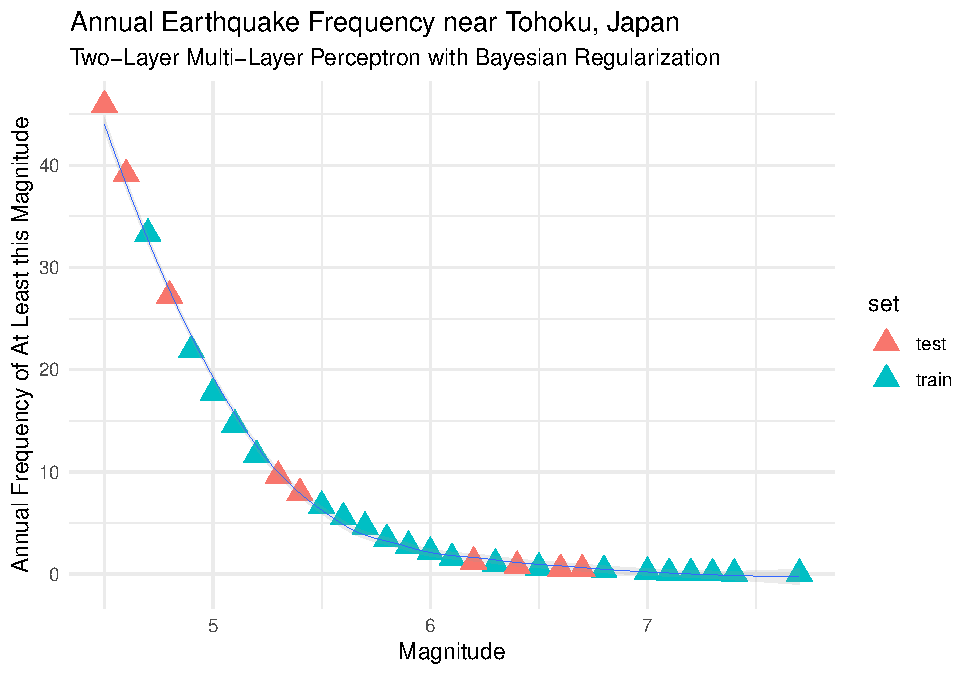
\includegraphics{Appendix_eq_files/figure-latex/unnamed-chunk-11-1.pdf}

\begin{Shaded}
\begin{Highlighting}[]
\FunctionTok{rbind}\NormalTok{(poissontable,mlptable\_cv,brnntable)}
\end{Highlighting}
\end{Shaded}

\begin{verbatim}
##                  Model    TestErr
## 1   Poisson Regression 0.03940496
## 3                  MLP 0.18594794
## 6                  MLP 0.29409940
## 9                  MLP 0.50040977
## 10                 MLP 0.31526324
## 20                 MLP 0.84218635
## 31                BRNN 0.26881221
## 61                BRNN 0.27750571
## 91                BRNN 0.27483569
## 101               BRNN 0.24656257
## 201               BRNN 0.19927502
\end{verbatim}

